\documentclass{article}
\usepackage[margin=0.8in]{geometry}

\usepackage[hidelinks]{hyperref}
\usepackage{minted}
\usepackage{pdfpages}
\usepackage{graphicx}
\usepackage{listings}
\usepackage{pdflscape}
\usepackage[caption=false]{subfig}

\lstset{
	numbersep=8pt, 
	frame = single, 
	framexleftmargin=15pt}

\begin{document}
\hypersetup{pageanchor=false}
\begin{titlepage} % Suppresses headers and footers on the title page
  \centering % Centre everything on the title page
  
  %------------------------------------------------
  %	Title
  %------------------------------------------------
  \vspace*{0.1\textheight}
  \large{EEL 5721 -- Reconfigurable Computing}\\
  \vspace{0.0025\textheight}
  
  \huge{Lab 0 -- VHDL Tutorial}
  \vspace{0.025\textheight} % Whitespace between the title and short horizontal rule
  
  \rule{0.3\textwidth}{0.4pt} % Short horizontal rule under the title
  \vspace{0.1\textheight} % Whitespace between the thin horizontal rule and the author name
  
  %------------------------------------------------
  %	Author
  %------------------------------------------------
  \small{By}\\
  \Large \textsc{Nathan Jessurun}\\% Author name
  \vspace{0.04\textheight}
  
  \vspace{0.10\textheight}
  \normalsize{
    \today
  }
  \vfill % Whitespace between the author name and publisher
  
  \rule{\textwidth}{0.4pt} % Thin horizontal rule
\end{titlepage}
\hypersetup{pageanchor=true}
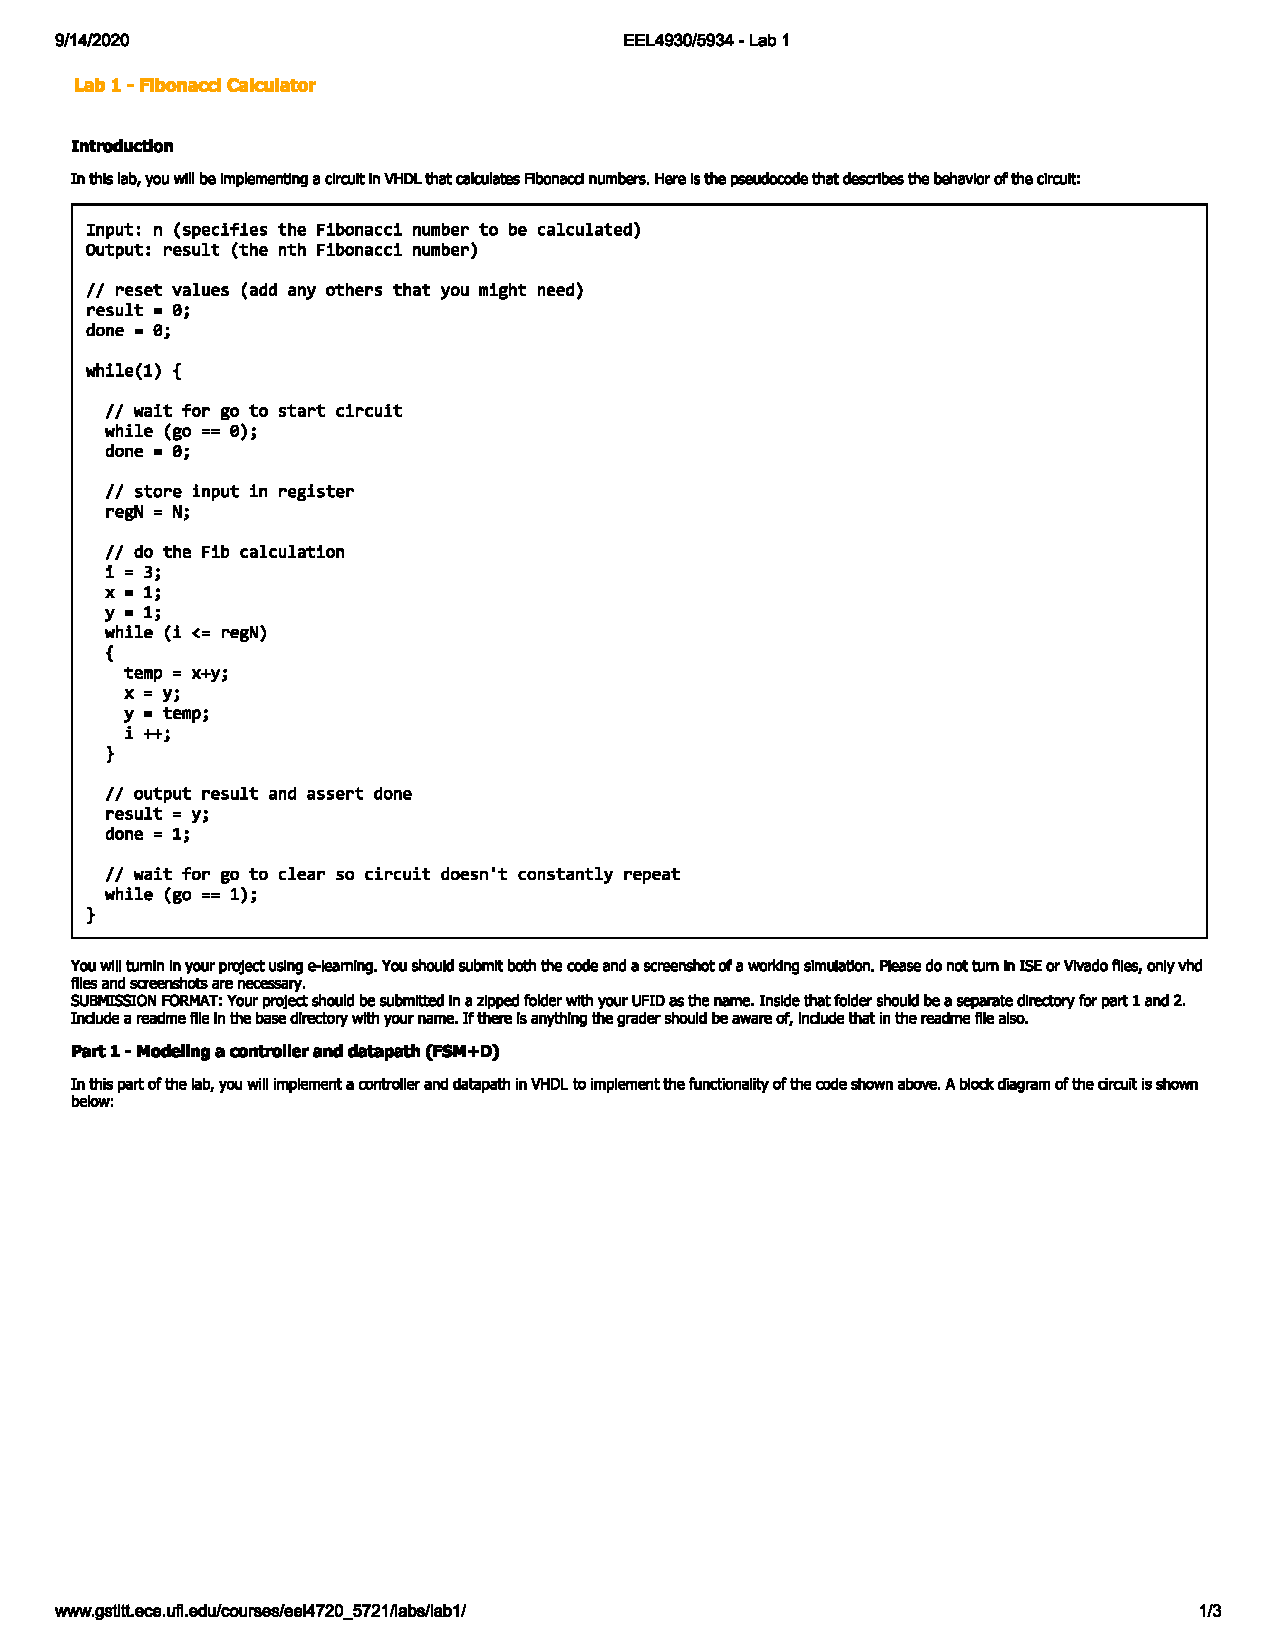
\includepdf[pages=-]{./lab}

\begin{landscape}
\section{Working Simulations}
\texttt{true\_fib} represents the output of a fibonacci function on input $n$ to assist in verifying the FSM output.
\begin{figure}[H]
	\centering
	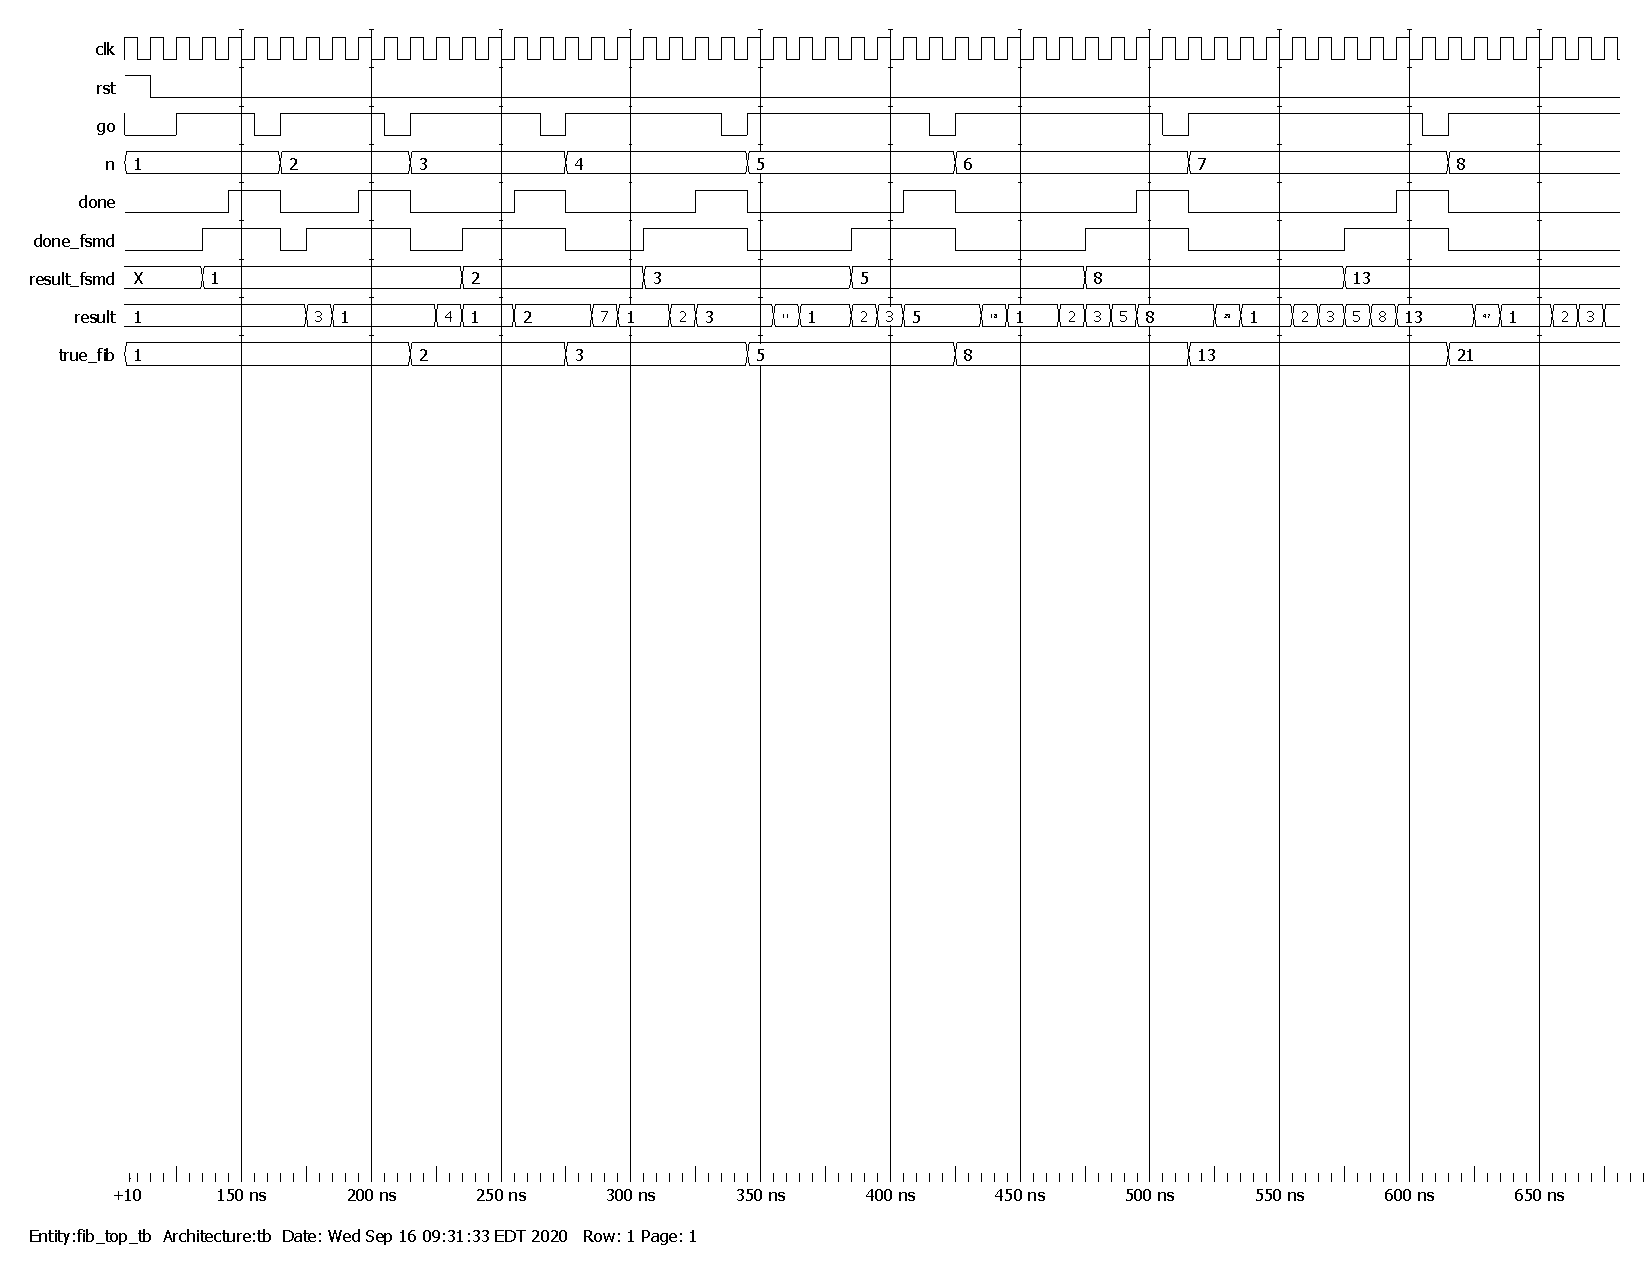
\includegraphics[width=\linewidth,clip,trim=0cm 15cm 0cm 0cm]{figures/simResults}
	\caption{`true\_fib' represents the fibonacci result for input $n$ to assist with verifying the FSM result}
	\label{fig:fsmplusdtb}
\end{figure}
\end{landscape}

\section{Design Size Comparison}
The number of LUTs required for FSM+D and FSMD designs are shown in Figure \ref{fig:sizecmp}.
Both implementations are similar in their underlying logic, so it makes sense their LUT sizes should be close to each other (22 vs. 32). However, the FSMD path used registers more liberally than the alternative approach. Rather than specifying muxes and register loads to determine behavioral logic, I chose to make $x$, $y$, and $i$ all come with additional \texttt{next} counterparts to greatly simplify the amount of vhdl code. Hence, it makes sense this design would feature a larger footprint.


\begin{figure}[!htbp]
	\centering
	\subfloat[]{%
		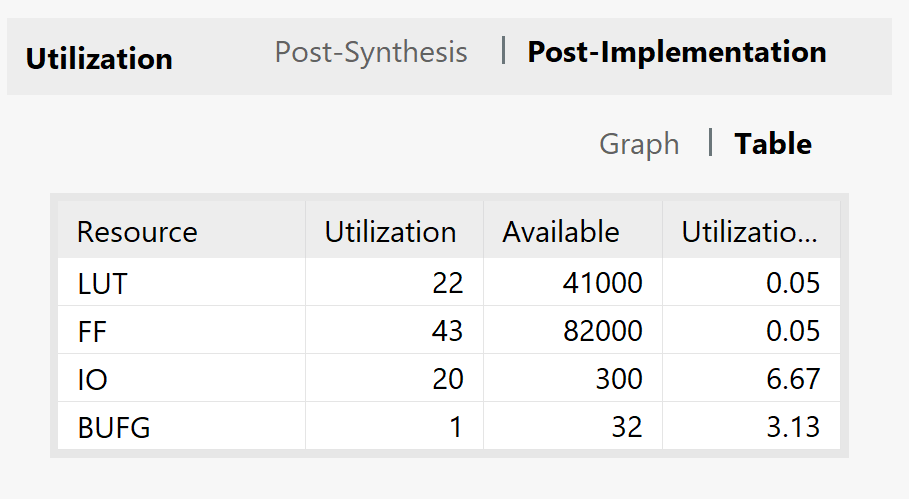
\includegraphics[width=0.48\linewidth]{figures/fsm_plus_d_size}%
	}
	\hfill
	\subfloat[]{%
		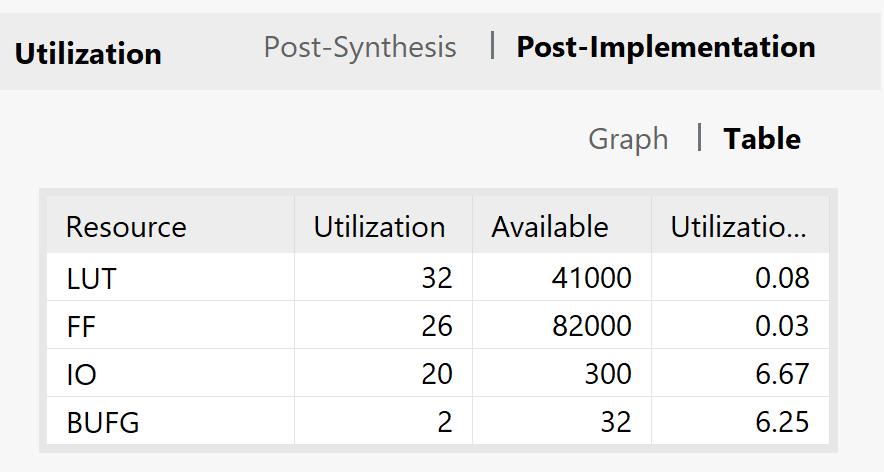
\includegraphics[width=0.48\linewidth]{figures/fsmd_size}%
	}
	\caption{Comparison of LUT sizes for FSM+D (left) and FSMD (right) implementations of a Fibonacci calculator.}
	\label{fig:sizecmp}
\end{figure}

\section{Code Listings}
Per instructions, all code files are zipped along with the project report.
\end{document}